\subsection{Baseline Methods}

\begin{table}
\centering
  \caption{Datasets}
  \begin{tabular}{|l|l|l|}
    % \toprule
    \hline
    Data set & \# features & \# instances\\ \hline
    USPS & 256 & 10,000\\ \hline
    MNIST & 780 & 60,000\\ \hline
    VIDEO & 100 & 5,000\\ \hline
    DVD & 200 & 30,000\\ \hline
    MUSIC & 300 & 30,000\\ \hline
    SYN01 & 100 & 10,000\\ \hline
    SYN02 & 200 & 20,000\\ \hline
    
%   \bottomrule
\end{tabular}
\label{tbl:datasets}
\end{table}

\begin{table*}[t]
\centering
\caption{Comparison of performance}
\label{tbl:performance}
\resizebox{1.4\columnwidth}{!}{%
\begin{tabular}{|l|l|l|l|l|l|}
\hline
Error Rate                & OTL    & HeMap-S & HeMap-L & MSDA-S & MSDA-L\\ \hline
USPS $\rightarrow$ MNIST  & 0.3231 & 0.3819  & 0.3904  & \textbf{0.2872} & 0.2996\\ \hline
MUSIC $\rightarrow$ DVD   & 0.3354 & 0.3606  & 0.3585  & 0.3291 & \textbf{0.3164}\\ \hline
VIDEO $\rightarrow$ MUSIC & 0.3801 & 0.4041  & 0.3972  & \textbf{0.3176} & 0.3202\\ \hline
VIDEO $\rightarrow$ DVD   & 0.3588 & 0.4028  & 0.4009  & \textbf{0.3235} & 0.3384\\ \hline
SYN01 $\rightarrow$ SYN02 & 0.3753 & 0.4183  & 0.4212  & \textbf{0.3350} & 0.3547\\ \hline
\end{tabular}
}
\end{table*}

To evaluate the effectiveness of our proposed our method MSDA, which uses embedding based methods for domain adaptation, we compare it with several state-of-the-art domain adaptation or online learning frameworks. Also, we applied two different variations of our method, which are MSDA-SVM and MSDA-LR. These two methods are different in a way that classifiers applied are SVM and Logistic Regression. The following paragraphs describe details of baseline methods.

\textbf{HeMap}. Heterogeneous Mapping (HeMap) projects data in two domains with correspondence onto a common latent space~\cite{shi2010transfer}. This method is designed as a batch training, which means both source and target data are offline. Also, this method requires class labels in the target dataset. We adapt HeMap into our problem by applying sliding windows. Meanwhile, two classifiers, SVM and LR, are also applied in this method as variations, which are referred as HeMap-S and HeMap-L respectively. 

\textbf{OTL}. Online Transfer Learning uses a co-regularized method to project target domain data into the source domain~\cite{zhao2010otl}. This method is applied in a supervised manner, which means that data in source domain are offline, while data in target domain are online. Furthermore, there is a strong assumption that features in source stream are a subset of those in target stream.

\subsection{Datasets}
\label{sec:datasets}




We use both synthetic and real-world datasets to evaluate our methods. As Table~\ref{tbl:datasets} shows, the first five datasets are publicly available, and the latter two synthetic datasets are generated by MOA~\cite{bifet2010moa}. 

\textbf{USPS}~\cite{hull1994database} and \textbf{MNIST}~\cite{lecun1998gradient} contain gray-scale images of hand-written digits collected from different sources. 
Each digit is size-normalized and centered in a fixed-size image, and each digit is a feature in these two datasets. Thus the number of features in two datasets are different due to the different resolution of the images.
In order to satisfy the concept drift assumption in this paper, we shift the concept of positive and negative classes in the middle of datasets. 
That is, in the first half of both USPS and MNIST, labels 0-4 represent ``-'' and labels 5-9 represent ``+'', while in the second half class labels 3-7 mean ``+'' and the rest class labels mean ``-''.

\textbf{MUSIC}, \textbf{DVD}, and \textbf{VIDEO} are text datasets generated by Amazon reviews based on product categories~\cite{blitzer2007biographies}. In these datasets, video has 5,000 of customer reviews, while MUSIC and DVD have 30,000 balanced customer reviews. Features are extracted directly from raw review text by implementing word2vec model trained by Google~\cite{mikolov2013efficient}. In order to use this data set in a binary classification setting, we label scores with ratings greater than 3 is defined as``+'', and those smaller than 3 are defined as ``-''. Scores that equals to 3 is discarded due to ambiguous polarity. Meanwhile, weighted average sentence embedding~\cite{arora2016simple} is applied to represent word vectors, which provide more weight to uncommon words.

\textbf{SYN01}, \textbf{SYN02} are synthetic datasets that are generated by MOA framework. These datasets are generated in a way that the number of features in SYN01 is 100 while that in SYN02 is 200, so that our domain adaptation assumption can be satisfied.

\subsection{Experiment Setup}
Our MSDA approach involves multiple parameters. We use $N_m = 400$ as our default setting in the experiment. Meanwhile, $\beta = 1$, $k = 4$, and $\tau = 0.1$ are selected to conduct our initial experiment here. The sensitivity of parameters will be discussed later in this section.

\subsection{Result Analysis}

\begin{figure*}[t]
   \centering
   \subfloat[][]{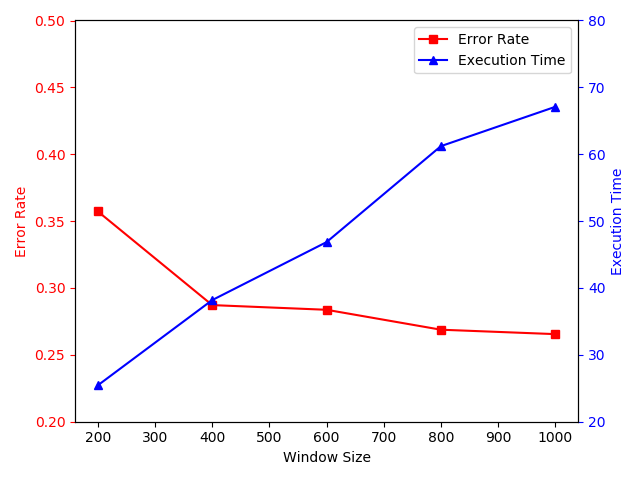
\includegraphics[width=.35\textwidth]{Figures/sen_window.png}} 
   \subfloat[][]{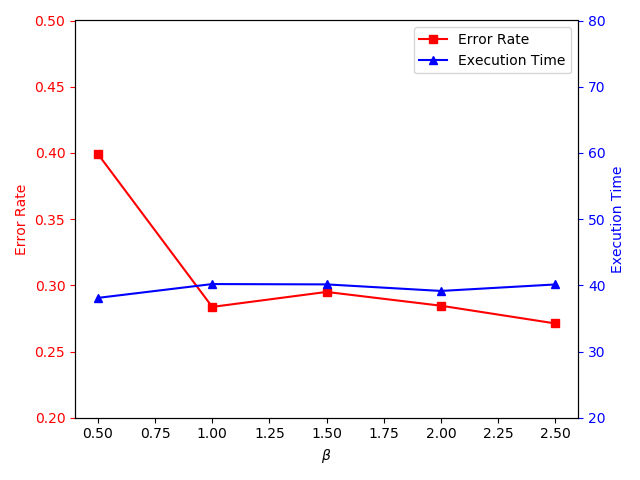
\includegraphics[width=.35\textwidth]{Figures/sen_beta.png}} \\
   \subfloat[][]{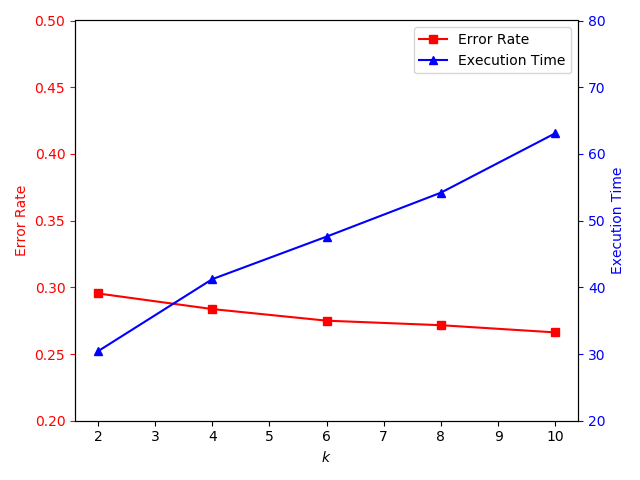
\includegraphics[width=.35\textwidth]{Figures/sen_k.png}} 
   \subfloat[][]{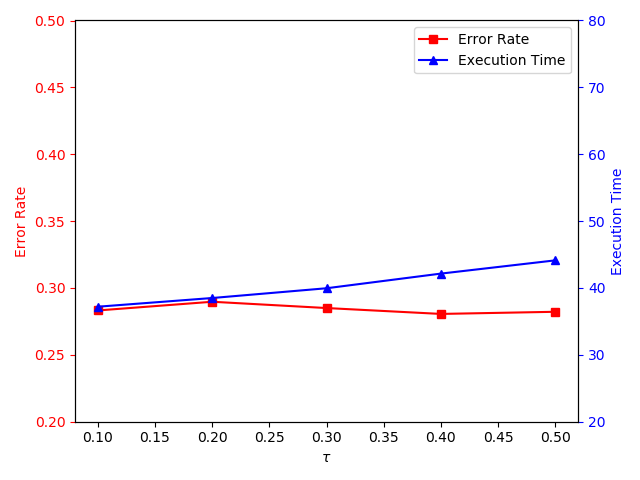
\includegraphics[width=.35\textwidth]{Figures/sen_tau.png}}
   \caption{Sensitivity Experiment Results of MSDA}
   \label{fig:sensitivity}
\end{figure*}


Table~\ref{tbl:performance} shows the average prediction error \% on the target stream $T$: $\frac{A_{wrong}}{m}$, where $A_{wrong}$ is the total number of instances identified incorrectly, and $m$ is the number of instances in the target stream. From this table, we can tell that MSDA-S outperforms all other competing methods on almost every dataset,except MUSIC $\rightarrow$ DVD. The reason here is because in other datasets information are transferred from low-dimensional to high-dimensional feature space while this dataset is reversed. Since the performance of the model can not be simply reversed, our method works better when adapting from small feature space to larger feature space. 

For example, the accuracy of OTA, HeMap-S and MSDA-S on USPS $\rightarrow$ MNIST are $32.31\%$, $38.19\%$ and $28.72\%$ respectively. 
We can see that our proposed method has better performance by a significant margin compared to baseline methods. The reason is that for OTL, the algorithm has a strong assumption that features in the source data are a subset of those in the target stream, which is not quite the case here.  
Text dataset used in this paper, such as reviews for VIDEO and DVD, would have overlapping features in terms of data distributions. However, not all features in VIDEO would exist in the DVD dataset in our settings. 
When it comes to HeMap, it also has its own shortcomings. HeMap is an offline method, which makes it not able to adapt the concept drift assumption in our problem. In this dataset specifically, the concept in the second half of data shifts from the first half of data (described in Section~\ref{sec:datasets}). Since we applied periodic updates every 4000 instances for the HeMap method, there is a delay on updating the model comparing our proposed MSDA-S approach.

\subsection{Sensitivity Analysis}
The results of our proposed method are further analyzed by tuning defined parameters $N_m$, $\beta$, $k$, and $\tau$. All experiments are conducted on USPS $\rightarrow$ MNIST dataset. In this section, we vary $N_m$ by setting it to \{200, 400, 600, 800, 1000\}, $\beta$ to \{0.5, 1, 1.5, 2, 2.5\},
$k$ to \{2, 4, 6, 8, 10\}, and  $\tau$ to \{0.1, 0.2, 0.3, 0.4, 0.5\} respectively.

First, the parameter that controls window size ($N_m$) is set to different values, and results are shown regarding how they affect MSDA approach in Figure~\ref{fig:sensitivity}. We can see that the average error decreases while the increasing window size, while the execution time increases with increasing window size. This is expected as we state that the execution time of MSDA depends on $N_m$. Based on this observation, we should choose a medium value so that both error rate and execution time could be balanced.

Second, $\beta$ determines the similarities between projected domains from both source and target stream. From Figure~\ref{fig:sensitivity}, we can tell that the error rate decreases significantly when $\beta$ increases from 0.5 to 1. If $\beta > 1$, the decreasing trend of error rate is becoming not significant. Also, we can see from the figure that the execution time regarding different $\beta$ remains similar in the experiment. Thus, we choose $\beta = 1$ as our recommended parameter here.

Third, considering the parameter that defines the dimension of latent feature space $k$. This parameter influence the model in both embedding and classification. In other words, this parameter determines how large the feature space is to apply our classifiers. From Figure~\ref{fig:sensitivity}, we can see that the performance of the model has improved marginally while the execution time increases dramatically as $k$ increases. Thus, we need to choose as small $k$ as possible, meanwhile we need to make sure that performance doesn't degrade. Thus, we choose $k = 4$ for our approach.

At last, we can see that for $\tau$, which controls the threshold for concept drift detection. In this case, the performance of model doesn't quite change when $\tau$ varies. Therefore, based on performance of execution time, we need to choose a smaller $\tau$. Hence, we select $\tau = 0.1$ in our model.

In all, those sensitivity experiments indicate that MSDA is sensitive to $N_m$ and $k$, while not quite sensitive to $\beta$ and $\tau$. 